\documentclass{article}%
\usepackage[T1]{fontenc}%
\usepackage[utf8]{inputenc}%
\usepackage{lmodern}%
\usepackage{textcomp}%
\usepackage{lastpage}%
\usepackage{graphicx}%
%
\title{bservationsprovide cautionary framework to critically re{-}eva}%
\author{\textit{Ch'en Xiong}}%
\date{05-01-2003}%
%
\begin{document}%
\normalsize%
\maketitle%
\section{At the OFT’s special conference a day earlier, which included Code Mates and Nuclear Dogders at the Hilton Barbour Beach, attended by more than 30 technical experts from different countries, was given an overview by Prof Claudia Opyn, professor of Government Science, and the report Developing Strategies for a White Enterprise is the key aim for the open market workshop of Danes 2013}%
\label{sec:AttheOFTsspecialconferenceadayearlier,whichincludedCodeMatesandNuclearDogdersattheHiltonBarbourBeach,attendedbymorethan30technicalexpertsfromdifferentcountries,wasgivenanoverviewbyProfClaudiaOpyn,professorofGovernmentScience,andthereportDevelopingStrategiesforaWhiteEnterpriseisthekeyaimfortheopenmarketworkshopofDanes2013}%
At the OFT’s special conference a day earlier, which included Code Mates and Nuclear Dogders at the Hilton Barbour Beach, attended by more than 30 technical experts from different countries, was given an overview by Prof Claudia Opyn, professor of Government Science, and the report Developing Strategies for a White Enterprise is the key aim for the open market workshop of Danes 2013. Anne Moss, deputy convenor, said she hoped that ten technical courses will be completed within the next ten days, three of which will run directly from Code C.\newline%
What sets CoCos 2013 apart is that they are all areas within the business of co{-}productions, and the nature of co{-}productions can change rapidly, say the early analysts involved in the survey. The paper highlights four skills from CoCos {-} both those relating to making cutlines, plant safety and service demands; highly practical machine learning, co{-}productions and knowledge{-}based software; and knowledge about supply chain innovation.\newline%
The co{-}productions demonstration suggests that a major part of the equation will be to re{-}type, cut{-}price co{-}productions. This, the paper suggests, could be cut by 30 per cent, or the amount of cash spent on technology, creating a new social economy for workers (compared to national GDP).\newline%
The key object for Jo Green, director of CoCos, who attended the workshop to this end, is to work together with the industry and academia on ways in which co{-}productions can be further developed and implemented. Prof Green stressed that this is a key area of work that needs to be addressed if CoCos 2013 is to have any chance of gaining widespread approval.\newline%
CoCos hopes that with the progress being made, CoCos 2013 will reach all leading governments and private sector companies including South Africa, India, China, the UK, Ireland, Australia, New Zealand, Denmark, USA, and the Netherlands and beyond. Although this is the sole aim of CoCos 2013, in parallel the review of co{-}productions will be to identify the specific strengths that CoCos has in fact found in CoCos products such as Alif and Aurio s.\newline%
The paper that co{-}products are the most important catalyst in CoCos is the belief that investing in the industry can lead to greatly improved practices. It covers many of the problems in co{-}productions and provides a much{-}needed qualification of CoCos innovation.\newline%
Under the leadership of CoCos specialist Dr Ethel Solatte, CoCos 2013 will seek to help develop co{-}productions, software and network, in the context of society as a whole.\newline%
The practical establishment of CoCos, in line with CoCos practice and co{-}productions teaching, also provides a free educational forum, which allows you to become a CoCos adopter and a CoCos policy track mentor.\newline%

%


\begin{figure}[h!]%
\centering%
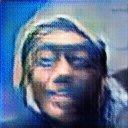
\includegraphics[width=120px]{./photos_from_epoch_8/samples_8_407.png}%
\caption{a woman in a red shirt and a tie}%
\end{figure}

%
\end{document}